
\section{\tikzname{} Interoperability}
\label{pgfplots:tikz:interoperability}

\PGFPlots{} uses \Tikz{}/\pgfname{} as its ``backend layer''. This implies that it
inherits most of \Tikz's graphical features and adds a lot of own stuff on top
of it. However, the coordinate systems of \Tikz{} and \PGFPlots{} do not match
up -- for good reason: \PGFPlots{} operates on logical (data) coordinates
whereas \Tikz{} operates on image coordinates.

Occasionally, one may want to synchronize both in order to generate a graphic.
In this context, ``synchronize both'' means that they really use the same
coordinate systems. This is far beyond the simple use case of ``enrich a
\PGFPlots{} picture by means of \Tikz{} annotations'', compare
Section~\ref{sec:pgfplots:annotations}.

Consequently, this section addresses the question how to match the coordinates
from \Tikz{} to \PGFPlots{} and vice versa. It explains how to match
coordinates and it discusses the necessary configuration.

There are a couple of keys in \PGFPlots{} which control the mapping of
coordinates. The purpose of these keys is to implement visualization
techniques, but they do things different than \Tikz{} (and they should). To
match coordinates with \Tikz{}, one needs the following aspects:
%
\begin{enumerate}
    \item Restrict your visualization type: a logarithmic axis simply may not
        fit into \Tikz{} (to be more precise: it may fit, but a \Tikz{} unit
        will correspond to a log unit in \PGFPlots).
    \item Configure matching unit vectors by means of the |x| and |y| keys.
        The default configuration of \Tikz{} is to use
        |x=1cm,y=1cm,z={(0,0)}|. Note that these settings are usually
        overridden by \PGFPlots{} in order to respect |width| and |height|
        (and |view| for three-dimensional axes).
    \item Disable the data scaling by means of |disabledatascaling|:
        \PGFPlots{} will internally apply linear coordinate transformations
        in order to provide the data range required for floating point
        arithmetics (using approximately floating point precision). Disabling
        the data scaling means to restrict yourself to the (small) data range
        supported by \Tikz{} -- but that's probably what you want in that
        case.
    \item Define |anchor| and position of the |axis|, probably using
        |anchor=origin,at={(0,0)}|. The |at={(0,0)}| configures \PGFPlots{}
        to place the axis at the \Tikz{} position |(0,0)| whereas
        |anchor=origin| means that \PGFPlots{} will place its data origin
        $(0,0,0)$ at the place designated by |at| (see
        Section~\ref{pgfplots:sec:align} for details).
    \item Make sure that the \PGFPlots{} axis contains the data origin
        $(0,0,0)$ in the displayed data range (i.e.\@ configure |xmin|,
        |xmax|, |ymin|, and |ymax| appropriately).

        Without this, the |anchor=origin| key required in the previous item
        will be truncated to the next coordinate which is part of the displayed
        range.
\end{enumerate}

\noindent Here is a simple example, first with \Tikz{}:
%
\begin{codeexample}[]
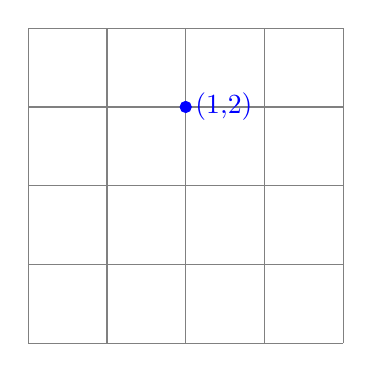
\begin{tikzpicture}
    \coordinate (Point) at (1,2);

    \draw [gray] (-1,-1) grid (3,3);
    \draw [blue,fill] (Point) circle (2pt)
        node [right] {(1,2)}
    ;
\end{tikzpicture}
\end{codeexample}
%
\noindent it displays a grid with $x,y\in[-1,3]$ and shows a node inside of it.
Now, we apply the keys discussed above to match this setting in \PGFPlots{}:
%
\begin{codeexample}[]
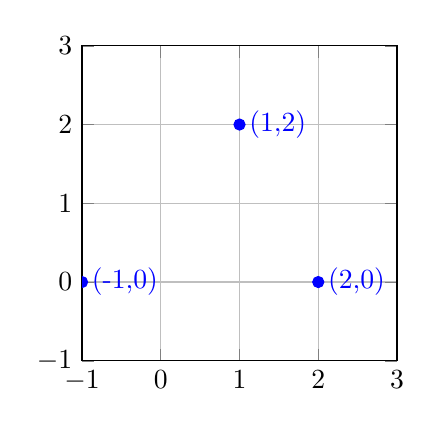
\begin{tikzpicture}
    \coordinate (Point) at (1,2);
\begin{axis}[
    % tell pgfplots to "grab" the axis at its
    % internal (0,0) coord:
    anchor=origin,
    % tell pgfplots to place its anchor at (0,0):
    % (This is actually the default and can
    % be omitted)
    at={(0pt,0pt)},
    % tell pgfplots to use the "natural" dimensions:
    disabledatascaling,
    % tell pgfplots to use the same unit vectors
    % as tikz:
    x=1cm,y=1cm,
    %
    % this is just as usual in pgfplots. I guess
    % it is only useful if (0,0) is part of the
    % range... try it out.
    xmin=-1,xmax=3, ymin=-1,ymax=3,grid=both,
]
    % this uses the point defined OUTSIDE of the axis
    \draw [blue,fill] (Point) circle (2pt)
        node [right] {(1,2)};

    % this uses a TIKZ coordinate (2,0) in the axis:
    \draw [blue,fill] (2,0) circle (2pt)
        node [right] {(2,0)};

    % this here will always work inside of an axis:
    \draw [blue,fill] (-1,0) circle (2pt)
        node [right] {(-1,0)};
\end{axis}
\end{tikzpicture}
\end{codeexample}
%
\noindent The example demonstrates several things: first, it defines a
coordinate in the enclosing |tikzpicture| and uses it inside of the |axis| (at
the correct position). Second, it uses the standard \Tikz{} coordinate |(2,0)|
inside of the |axis|, and it is placed at the expected position. Third, it uses
the approach provided by \PGFPlots{} by using the |axis cs| to designate a
coordinate (this last approach does also work without the coordinate matching).

Here is an example which inserts a \PGFPlots{} graphics correctly into a
|tikzpicture|:
%
% \usepgfplotslibrary{patchplots}
\begin{codeexample}[]
% requires \usepgfplotslibrary{patchplots}
\begin{tikzpicture}
    \begin{axis}[
        % tell pgfplots to "grab" the axis at its internal (0,0) coord:
        anchor=origin,
        % tell pgfplots to place its anchor at (0,0):
        % (This is actually the default and can be omitted)
        at={(0pt,0pt)},
        % tell pgfplots to use the "natural" dimensions:
        disabledatascaling,
        % tell pgfplots to use the same unit vectors as tikz:
        x=1cm,y=1cm,
        %
        hide axis,
    ]
        \addplot [patch,patch type=coons,
            shader=interp,point meta=explicit]
        coordinates {
            (0,0)      [0] % first corner
            (1,-1)     [0] % bezier control point between (0) and (3)
            (4,0.7)    [0] % bezier control point between (0) and (3)
            %
            (3,2)      [1] % second corner
            (4,3.5)    [1] % bezier control point between (3) and (6)
            (7,2)      [1] % bezier control point between (3) and (6)
            %
            (7,1)      [2] % third corner
            (6,0.6)    [2] % bezier control point between (6) and (9)
            (4.5,-0.5) [2] % bezier control point between (6) and (9)
            %
            (5,-2)     [3] % fourth corner
            (4,-2.5)   [3] % bezier control point between (9) and (0)
            (-1,-2)    [3] % bezier control point between (9) and (0)
        };
    \end{axis}

    % this requires pgf 2.10
    \begin{scope}[every node/.style={circle,inner sep=2pt,fill=black}]
        \node [pin=140:first] at (0,0) {};
        \node [pin=second]    at (3,2) {};
        \node [pin=45:third]  at (7,1) {};
        \node [pin=0:fourth]  at (5,-2) {};
    \end{scope}
\end{tikzpicture}
\end{codeexample}
%
\noindent The example employs one of the |patch| plots of the |patchplots|
library. Since these graphical elements typically require depth information
(|z buffer|ing) and color data (|point meta|), they are only available inside
of \PGFPlots{}. However, the configuration above ensures that coordinates match
one-to-one between \PGFPlots{} and \Tikz{}. The |hide axis| flag disables
anything of \PGFPlots{}, so only the visualized |patch| plot
remains.\footnote{Note that the $(0,0,0)$ coordinate of \PGFPlots{} is part of
the data range here.}
